\section{Related Work \& Theoretical Grounding}

The first step towards answering the questions mentioned before, as well as ultimately contributing to the research field, is thorough scouting of related work. This allows for both a high-level overview of the state-of-the-art research in the field of play and a deeper insight into comparable research specific to the context at hand.

The structure of that scouting is going to be defined by what results are needed as a foundation for the next steps of research within this thesis. As the overall research topic revolves around investigating the intersection between the fields of software development and play, this state-of-the-art investigation has to reflect that. Thus, there is a need for researching related work in those two different areas of research. One of those two is play, where it is crucial to gain an understanding of what play entices, how it can be defined and how it can be leveraged and enabled in different contexts. One of these contexts is the second area of research being investigated in this thesis: Software development in general and onboarding onto software development projects specifically. This then serves as the theoretical grounding for all further work. To gain a more complete understanding of the intersection of play and software development one additional step is required, though: Analyzing the state of play in software development, where it is used, how and to which effect. Ultimately this results in a three-fold approach to research into related work:

\begin{enumerate}
  \item{Research into the state-of-the-art of play as a research field}
  \item{Contextual considerations and peculiarities of onboarding in software development projects}
  \item{Discovery of existing attributes of play in software development}
\end{enumerate}

As mentioned these three parts serve as the theoretical foundation for the playful design guidelines, as well as the study later on. Therefore, special attention is given to research that informs both of those as well. This could mean, discovering design implications that are mentioned in the given literature or theoretical grounding for the preparation and the study itself.

\subsection{Play}

The concept that underlies the work done within this thesis is the concept of play. But what is it really, how could you define play, what does it entice, and how would you approach researching it? Before even trying to answer these questions, it is paramount to clarify why play would even be a good candidate for this thesis' research. Play in itself is ever-present and most importantly inherent to humans. This is displayed quite well in children, where e.g., Fenson \& Schell describes children exploring their world through playing, without having explicitly learned to do it: \enquote{It is largely through their playful transactions with people and objects that they gain information about physical and social aspects of their environment} \cite{fenson1985origins}. Baldwin et al. as well have found that children as young as 9 months were able to draw simple inferences about non-obvious object properties after brief exploration phases with those objects \cite{baldwin1993infants}.

\subsubsection{The Origins of Research into Play}

This does not necessarily fully translates to the context investigated in this thesis. Additionally, there might be differences in how children play vs. how adults play. However, it shows that play is innate to humans. There are important distinctions in how that manifests though, which is going to be a further point of discussion in this chapter. To get to that point of discussion play has to be defined in some way. As already mentioned there is no single, concise definition of what play is in research. Its meaning evolved and is subject to influences from the respective paradigms and worldviews behind its different definitions. Independently of these different definitions, there is a need to define a starting point to discuss the meaning of play.

Fortunately, this starting point is very well-defined in the area of play. Johan Huizinga marked said point clearly with his book \textit{Homo Ludens: A Study of the play-Element in Culture} \cite{huizinga2020homo}. Within it, he argues in great detail about characteristics of play. He describes where the differences towards other human behaviors lie and grounds it within a plethora of cultural examples throughout history. His main contribution that influenced a great amount of subsequent research are five characteristics attributed to play. While these are not without their fair share of critique, as we are going to find out later, they certainly are important to describe the origins of research in play.

Before diving deeper into these characteristics it is important to note that Huizinga himself constricted his definition to the relation of culture and play: \enquote{Since our theme is the relation of play to culture we need not enter into all the possible forms of play but can restrict ourselves to its social manifestations} \cite[p. 7]{huizinga2020homo}. Therefore, he excludes \enquote{the more primitive play of infants and young animals} \cite[p. 7]{huizinga2020homo} and limits himself on \enquote{contests and races, of performances and exhibitions, of dancing and music, pageants, masquerades, and tournaments} \cite[p. 7]{huizinga2020homo}. It is important to set the following description of his findings into context based on that. This description starts with the first attribute of play:

\begin{quote}
  \textit{Here, then, we have the first main characteristic of play: that it is free, is in fact freedom.}

  \footnotesize{Johan Huizinga, \cite[p. 8]{huizinga2020homo}}
\end{quote}

Naturally, the first follow-up question to this statement is the definition of freedom or free in this context. What does he mean with play being free or freedom itself? Gladly this is clearly described in his work as well: \enquote{First and foremost [...] all play is a voluntarily activity play to order is no longer play: it could be at best a forcible imitation of it} \cite[p. 7]{huizinga2020homo} and even though it is mentioned that play by instinct (as e.g. children play) is not necessarily voluntary play, the enjoyment can be freedom. There are two \enquote{sub-characteristics} as well that are notable here: \enquote*{play is superfluous} and \enquote*{it is done at leisure, during "free time"} \cite[p. 8]{huizinga2020homo}. Overall, Huizinga characterizes play as something that can not be imposed upon someone but has to be intrinsically engaged with. Moving onto the second characteristic, Huizinga writes:

\begin{quote}
  \textit{[...] play is not "ordinary" or "real" life. It is rather a stepping out of "real" life into a temporary sphere of activity with a disposition all of its own [... play is distinct from "ordinary" life both as to locality and duration. [...] It is "played out" within certain limits of time and place. It contains its own course and meaning}

  \footnotesize{Johan Huizinga, \cite[p. 8-9]{huizinga2020homo}}
\end{quote}

What Huizinga illustrates is that play and playful activities allow the player to experience a space disconnected from \textit{real} life. This allows the player to fully indulge in the activity and its \textit{artificial} context. This description was greatly influential in later research. It marked the first advance into the idea of a \textit{Magic Circle}. This \textit{Magic Circle} is in \enquote{a very basic sense, the magic circle of a game is where the game takes place. To play a game means entering into a magic circle, or perhaps creating one as a game begins} \cite[p. 95]{salen2004rules}. Criticism emerged concerning that notion, though. Consalvo for example mentions that players always bring outside knowledge about games and gameplay into gaming situations \cite[p. 415]{consalvo2009there}. Copier on the other hand proposes to go beyond the magic circle and rather view games from a network perspective \cite[p. 11]{copier2007beyond}. Nonetheless, it still holds relevance for discussing the different contexts of play and the real or ordinary. The fourth characteristic of play then is concernel with what play creates in an \textit{ordinary} world, \enquote{it creates order, is order. Into an imperfect world and into the confusion of life it brings a temporary, a limited perfection} \cite[p. 10]{huizinga2020homo}. This is closely connected to the idea of the magic circle as well.

Positively framed this means that \enquote{play casts a spell over us; it is "enchanting", "captivating"} \cite[p. 10]{huizinga2020homo}, that the order it creates within itself leads to a certain kind of immersion. On the other hand, as Huizinga points out: \enquote{The least deviation from it "spoils the game", robs of its character and makes it worthless} \cite[p. 10]{huizinga2020homo}. That kind of interpretation of play also leads to Huizinga's emphasis on the rules of play. He writes that \enquote{all play has its rules} and further \enquote{the rules of a game are absolutely binding and allow no doubt [...] as soon as the rules are transgressed the whole play-world collapses} \cite[p. 11]{huizinga2020homo}. This is a very black-and-white perspective on rules of play and its order. Other attempts at defining play put this into different perspectives. Ultimately though, Huizinga argues on the importance of rule sets as prerequisites for play itself. How important these are in the context of this thesis, is going to be subject of discussion throughout this chapter. Lastly, the fifth characteristic described by Huizinga is, connected to the \textit{materiality of play}, describing that it \enquote{is an activity connected with no material interest, and no profit can be gained from it} \cite[p. 13]{huizinga2020homo}.

After laying out in detail the starting point of play as a research field, it is extremely important to reflect on how these perspectives changed over time. Only by doing that a coherent picture of what makes play can be painted and later built upon. As mentioned before several points of critique emerged over time, some of which are going to be reflected on in the following.

To do this, Huizinga's work (as well as its critique) has to be set into historical perspective. Definitions of play before often described \enquote{play as a tool for the satisfaction of a biological or social need} \cite{rodriguez2006playful}. These \textit{function-centered theories} also assume that \enquote{playing could in theory have been replaced by some other behavioral technique capable of fulfilling the same function} \cite{rodriguez2006playful} and therefore \enquote{any function-centered theory necessarily fails to explain why people play} \cite{rodriguez2006playful}. These considerations ultimately lead Huizinga to fully reject \textit{function-centered theories} and use comparative description rather than quantitative methods to argue in favor of his definition of play \cite{rodriguez2006playful}.

Drawing a distinct line towards these theories was important in the historical context of the work. Completely disregarding these functional theories might not be reasonable either, though. In order to gain a holistic grasp on what play is, both the intrinsic, ludic experience and the extrinsic social functions, biological needs and functional means have to be taken into account. This especially rings true in the context of this thesis, where the intrinsic desire to playfully explore is combined with an extrinsic goal of onboarding onto software development projects. Ultimately a broader perspective on play is needed, to inform such an approach.

There are other points of critique towards Huizinga as well. Hector Rodriguez mentions this in regard to the \textit{irrationality} of play:

\begin{quote}
  \textit{Huizinga also contents that playing is in some sense and "irrational" activity. Taken at face value, however, this assertion is patently false. Many games depend on strategic thinking and other forms of logical thought}
  \footnotesize{Hector Rodriguez, \cite{rodriguez2006playful}}
\end{quote}

As discovered earlier Huizinga emphasizes undoubted rules and clear boundaries as essential to play. Rodriguez counters this by mentioning that uncertainty is essential to play and can even be used as a generative source. Further, he proposes to \enquote{begin designing frameworks for actions that may or may not be considered playful} \cite{rodriguez2006playful}.

However, Rodriguez also mentions that Huizinga can be read rather as an approximation than an advancement of rigid definitions \cite{rodriguez2006playful}.

What can be criticized as well is Huizinga's \enquote{apparent blindness to the importance of politics, which they regard as particularly indefensible, considering the troubled times in which he lived and wrote} \cite[p. 84]{anchor1978history}. It has to be mentioned, though, that aside from \textit{Homo Ludens}, Huizinga was well aware of the importance of politics in his other work \cite[p. 85]{anchor1978history}.

A possibly important point though, especially regarding this thesis, is the connection of serious and playful activities. Here, Huizinga shows a certain kind of ambiguity through arguing that play does \textit{not} exclude seriousness, while simultaneously painting a sharp line between the two categories of play and seriousness \cite[p. 87]{anchor1978history}. Ultimately it can be concluded that there is valid critique towards Huizinga. These mainly arose due to misconceptions and ambiguity on Huizinga's part. Therefore, it is necessary to advance into other perspectives on play and reflect on other stances towards defining and describing play.

\subsubsection{Other Perspectives on play}

Due to the shortcomings or sometimes ambiguous arguments by Huizinga more perspectives on play emerged. Especially notable ones, were brought forth by Ian Bogost \cite{bogost2007persuasive}, Bernard Suits \cite{suits2020grasshopper} and Brian Sutton-Smith \cite{sutton2009ambiguity}. In the following the key points of their works are going to be laid out and reflected upon, starting with Suits' work, specifically \textit{The Grasshopper: Games, Life and Utopia} \cite{suits2020grasshopper}.

In this work Suits tries to define what games and playing games means. To arrive at such a definition he creates a fictional \textit{socratic dialogue} (see e.g., \cite{berlin2004methodology}) where he uses dialectical argumentation to arrive at a series of definitions. In essence the definition of \textit{playing a game} for Suits is:

\begin{quote}
  \textit{To play a game is to attempt to achieve a specific state of affairs [prelusory goal], using only mean permitted by rules [lusory means], where those rules prohibit use of more efficient in favour of less efficient means [constitutive rules], and where the rules are accepted just because they make possible such activity [lusory attitude] [...] playing a game is the voluntary attempt to overcome unnecessary obstacles.}

  \footnotesize{Bernard Suits, \cite[p.35]{suits2020grasshopper}}
\end{quote}

This definition itself is widely cited, but the actual dialogue behind is often disregarded -- as Mitchell describes it. Mitchell specifically mentions the \enquote{productive ambiguities of the text, particularly with regard to the relationship between games and society} \cite{mitchell2020reconsidering} as under-represented. And rather than arriving at \enquote{apparently universal truths [...] it situates these truths in social context. The text is therefore useful for anyone concerned with the social or political dimensions of games} \cite{mitchell2020reconsidering}. While this is not the focus of the research within this thesis, these definitions are important to mention due to their relevance in the field. Still there is additional criticism on this definition, e.g., by Back, who writes:

\begin{quote}
  \textit{His definition of game playing has some obvious flaws. For instance, it decrees that a game cannot use the most efficient means to win. But why cannot we have a race in this way that uses the fastest means of transport and even allows disabling other racers}

  \footnotesize{Allan Back, \cite[p. 5]{back2008paper}}
\end{quote}

Despite these criticisms, the definition still holds value. It served as a point of discussion for future scholars, as can be especially seen when investigating Sicart's work. For this thesis specifically, there are some aspects worth elaborating on in order to inform the study down the line. The prelusory goal for example is something that has to be kept in mind throughout the following study. This goal, as Suits describes it, should be achieved by a rule set (lusory means \& constitutive rules). Within the context of this study constitutive rules play a special role. It could be argued that the most efficient software development onboarding (at least on a source code level) consists of interacting directly with said source code. Therefore, a rule set could hinder onboarding on that level, which is why that is a topic of interest going into the practical study.

Overall though, Suits' definitions were expanded upon greatly. Thus, it is a vital part of the history of research into play, albeit less vital for the informed implementation of the subsequent study. A perspective on play that might be able to serve as a foundation for such an endeavor, is Brian Sutton-Smiths body of work, especially \textit{The Ambiguity of play} \cite{sutton2009ambiguity}.

Staying within the theme of an ambiguous approximation of defining play, Sutton-Smith tries to approach the topic by dissecting \enquote{the rhetorics that are marginal to play \cite[p. VII]{sutton2009ambiguity}}. In this context \textit{rhetorics} can be defined as \enquote{being a persuasive discourse [...] to persuade others of the veracity and worthwhileness of their beliefs} \cite[p. 213]{wein2000suttonreview}. The work itself consists of the explanation of seven different rhetorics, described hereafter, as interpreted and condensed by Wein, as \enquote{the hypothesis presented here is complicated and abstruse, the proof complex and convoluted.} \cite{wein2000suttonreview}:

\begin{enumerate}
  \item{\enquote{\textbf{play as progress}, in which it is believed that "animals and children, but not adults adapt and develop through play"} (\cite[p. 8]{sutton2009ambiguity} as cited by \cite[p. 213]{wein2000suttonreview})}
  \item{\enquote{\textbf{play as fate}, focusing on games of chance which is in total contrast to play as progress} \cite[p. 213]{wein2000suttonreview}}
  \item{\enquote{\textbf{play as power} [...] is a way to represent conflict and to reinforce status} \cite[p. 213]{wein2000suttonreview}}
  \item{\enquote{\textbf{play as identity}: "usually applied to traditional and community celebrations and festivals} \cite[p. 10]{sutton2009ambiguity}" \cite[p. 213]{wein2000suttonreview}}
  \item{\enquote{\textbf{play as the imaginary} including all improvisions and literature} \cite[p. 213]{wein2000suttonreview}}
  \item{\enquote{\textbf{play applied to the self}, in which play is solely as a source of gratification or escape for its individual participants} \cite[p. 213]{wein2000suttonreview}}
  \item{\enquote{\textbf{play as frivolous}, which focuses on the foolery of play, its undermining of the work ethic, and its reflexivity} \cite[p. 213]{wein2000suttonreview}}
\end{enumerate}

Upon close inspection, there are a lot of important layers to unfold within each of those rhetorics. Concerning the context at hand though, there is little intersection and some contradiction on the utilization play within a professional software development environment. Especially the statement that adults do not develop through play, explicitly contradicts the notion of a playful learning experience in an onboarding process. Additionally, an undermining of the work ethic is not something research in this thesis strives for, arguably the contrary. And while the other rhetoric approaches explore important aspects of play and culture and the self, these are less applicable to the research fields within this thesis. Due to the additional, inherent ambiguity of the field, it is hard to derive informed design decisions from Sutton-Smith's work. Similar to Suits it rather gives more nuance to an approximated definition of play. This is only tangentially useful for the research goals of this thesis. On a positive note though, especially Miguel Sicart referenced and expanded a lot on Sutton-Smith's work. Before we are able to get into Sicart's work there is one more important contributor to the play research body that is necessary to mention: Ian Bogost.

Starting with \textit{Persuasive Games}, the central concept Bogost introduced was \textit{Procedural Rhetoric}, which is a type of rhetoric tied to how computers are functioning. More specifically it is a combination of the procedurality of computing in general and rhetorics as a mode of persuasion or in Bogost's own words: \enquote{Procedural rhetoric is the practice of persuading through processes in general and computational processes in particular} \cite[p. 3]{bogost2007persuasive}. In his book he argues that video games are uniquely positioned to leverage this power to persuade by presenting examples from three different areas, politics, advertising and learning \cite{bogost2007persuasive}.

Between those, the area of learning is of importance for this thesis. Before elaborating on that area though, there is additional clarification needed on the meaning of procedurality and rhetorics as Bogost defines it.

Starting with the term procedural, Murray's definition is used by Bogost. \enquote{Murray uses the term procedural to refer to the computer’s "defining ability to execute a series of rules." (as cited in \cite[p. 4]{bogost2007persuasive})}. Further, he explains that \enquote{Procedural systems generate behaviors based on rule-based models; they are machines capable of producing many outcomes, each conforming to the same overall guidelines} \cite[p. 4]{bogost2007persuasive}, which serves exceptionally well as a foundation for a rule set described by most of the preceding researchers in the area -- or as Bogost formulates it: \enquote{Because computers function procedurally, they are particularly adept at representing real or imagined systems that themselves function in some particular way} \cite[p. 5]{bogost2007persuasive}. Rhetoric on the other hand is described as a means of persuasion. Bogost describes the evolution from oral rhetorics of the early greek philosophers to visual rhetoric and finally arrives at the term coined by him. Where this gains relevance for this thesis is in its application in so-called \textit{persuasive games}. These are games that utilize the already addressed procedural rhetorics. Bogost presents multiple different examples of such games \cite[p. 46-53]{bogost2007persuasive} and thoroughly explains how certain game mechanics display aspects of such rhetoric.

An example that is brought up, is the game \textit{Tax Avoiders}, where a rather simplistic game mechanic and visual language is used to reach a goal removed from the game itself which in essence is just a jump-and-rum game. In this case, the player is trying to avoid enemy sprites representing tax agents and is able to use certain tax-avoidance measures between levels. Here the game \enquote{mounts an interesting and relatively complex procedural rhetoric about tax avoidance strategies} \cite[p. 52]{bogost2007persuasive}.

In the area of interest for this thesis -- Learning -- Bogost acknowledges that it is hard to define if video games can be educational, as the question: \textit{What does educational mean?} is hard to answer definitively \cite[p. 233]{bogost2007persuasive}. He further outlines two dominating, contemporary views on education. Those two are being influenced by a behaviorist worldview on one side and a constructivist on the other side. Bogost elaborates on the deficiencies of both when it comes to video games as educational tools. Behaviorists could argue that games can serve as a tool to learn about real-world models, e.g., playing \textit{Microsoft Flight Simulator} to learn about flying aircraft. This does not mean playing such a game makes you proficient enough in flying a real aircraft \cite[p. 238]{bogost2007persuasive}. Bogost calls this a \textit{simulation gap}, \enquote{the breach between the game's procedural representation of a topic and the player's interpretation of it} \cite[p. 238-239]{bogost2007persuasive}. But the constructivist approach is not without flaws as well. From its \enquote{perspective, video games teach abstract principles that service general problem-solving skills and learning values} \cite[p. 239]{bogost2007persuasive}. This view on the other hand neglects \enquote{video games’ ability to cultivate higher-order thinking skills} \cite[p. 240]{bogost2007persuasive}. Bogost's answer to this dilemma is the idea that:

\begin{quote}
  \textit{Videogames do not just offer situated meaning and embodied experiences of real and imagined worlds and relationships; they offer meaning and experiences of particular worlds and particular relationships. The abstract processes that underlie a game may confer general lessons about strategy, mastery, and interconnectedness, but they also remain coupled to a specific topic}

  \footnotesize{Ian Bogost, \cite[p. 241]{bogost2007persuasive}}
\end{quote}

In essence, this means that, while video game knowledge cannot be translated 1:1 to real-world knowledge, it might be able to educate about particular topics -- such as software development and onboarding in the case of this thesis (which is going to be subject of discussion going forward). What has to be mentioned though, is that \enquote{Video games teach biased perspectives on how things work} \cite[p. 260]{bogost2007persuasive} which is exactly why additional research is needed in order to explore its usage in the context of this thesis.

\subsubsection{A Contemporary View on Play}

Up until this point, we have discovered that a single, unified definition of play and playfulness does not exist. Arguably this is the only constant throughout the history of its research. This does not necessarily mean, that there are only conflicting perspectives on what play is. It rather means that there is a large number of different perspectives on what it entails, each being valuable to explain a certain aspect of it.

That does make it hard to derive actual implications for an informed design. An attempt to at least formalize a way of thinking about play, was done by Miguel Sicart. It is based upon and references much of what came before. His work \textit{Play Matters} was regarded positively upon publishing and is widely cited in the field on several occasions. Other works that reference it include topics such as social media \cite{hjorth2019understanding}, the mischief and antagonism on the internet \cite{phillips2018ambivalent}, or video games as culture \cite{daniel2018video}, and digital leisure \cite{spracklen2015digital}. The broadness of these sources show the applicability of Sicart's work in a number of different contexts. The specific applicability in this thesis' context is subject to discussion hereafter. What is also subject of discussion is the general perspective on play that Sicart offers. Ultimately the questions that should be answered  regarding his work, are:


\begin{itemize}
  \item{What's the essence of Sicart's definition or explanation of play?}
  \item{Where does Sicart's perspective extend upon or differ from previous research?}
  \item{Is this a valid theoretical grounding for the research within this thesis?}
\end{itemize}

Starting with the first of those questions, Sicart himself states that \enquote{play, like any other human activity, is highly resistant to formal understanding} \cite[p. 2]{sicart2014play} -- Therefore he is trying to understand play and why it matters, rather than formally defining it, a take that seems to be reasonable coming from the historically very diverse -- \textit{and ambiguous} -- approaches to such a definition. Sicart then starts trying to do so by opening with the statement: \enquote{To play is to be in the world. playing is a form of understanding what surrounds us, and a way of engaging with others.} \cite[p. 1]{sicart2014play}. Further, he positions his work as an extension of the canon of Huizingan play, while simultaneously being \textit{Post-Huizingan} in some points, as we are going to elaborate on in the subsequent paragraphs. Sicart also draws a sharp line to other perspectives on play that are focused on games in particular:

\begin{quote}
  \textit{Instead of deriving an understanding of play from a particular object or activity, like war, ritual, or games, I see play as a portable tool for being. It is not tied to objects but brought by people to the complex interrelations with and between things that form daily life.}

  \footnotesize{Miguel Sicart, \cite[p. 2]{sicart2014play}}
\end{quote}

If its meaning cannot be derived that way, another approach is necessary to explain why play matters and what it entails. Similar to how Sutton-Smith and Huizinga structured their attempt on explaining play, Sicart goes on to describe certain aspects of play. Starting with how \enquote{\textbf{play is contextual}} \cite[p. 6]{sicart2014play} and how \enquote{play happens in a tangled world of people} \cite[p. 6]{sicart2014play}. This network -- or play context -- is further defined as \enquote{the network of things, people, and places needed for play to take place} \cite[p. 7]{sicart2014play}. What is also mentioned in the course of this statement, is the idea of spaces of play and playgrounds. These are vital concepts within Sicart's book and hugely important for the research design that follows later on and therefore explained in more detail at that point.

The second aspect of play that is mentioned, is that \enquote{\textbf{play is disruptive} [...] When it takes over the context in which play takes place, it breaks the state of affairs} \cite[p. 14]{sicart2014play}. This allows for different outcomes in different situations, from disrupting a context for \enquote{simple} enjoyment to going beyond that and by appropriation revealing \enquote{the inner workings of the context we inhabit} \cite[p. 15]{sicart2014play}. This claim is of great importance regarding this thesis. It directly relates to what we want to achieve by combining the field of play with software development -- Revealing the inner works of software development projects respectively the surrounding context.

Another aspect of play proposed by Sicart is the idea that \enquote{\textbf{play is autotelic}--an activity with its own marked duration and spaces and its own conditions for ending} \cite[p. 16]{sicart2014play}. This might relate to previous research in this field, for example the already addressed \textit{magic circle} wherein play happens, and the clearly defined rule sets seemingly necessary for play. Sicart distances himself from such clear-cut boundaries, he writes \enquote{the boundaries of autotelic play are not formally rigid; there is no clear demarcation between the world of game and the world at large} \cite[p. 16]{sicart2014play}. Here we can observe a connection to what Bogost stated, concerning video games as educational tools. While the \textit{game world} is markedly different from the \textit{world at large}, certain concepts and systems do translate to this \textit{game world}. Sicart extends on this idea in this case, by verbalizing the ability of play to blur the lines between those worlds:

\begin{quote}
  \textit{We play by negotiating the purposes of play, how far we want to extend the influences of the play activity, and how much we play for the purpose of playing or for the purpose of personal expression}

  \footnotesize{Miguel Sicart, \cite[p. 16]{sicart2014play}}
\end{quote}

Important to note here is Sicart's addition that this negotiation happens constantly. Further, the purpose of play can change midway through activities. Because of that, it is even more relevant to understand in which context play happens and how such spaces can appropriate play.

Sicart further argues that \enquote{\textbf{play is creative}, in that it affords players different degrees of expression inherent in the play activity itself} \cite[p. 17]{sicart2014play}. He also states that it is \enquote{the act of creatively engaging with the world, with technologies, contexts, and objects, from games to toys to playgrounds, exploring them through ludic interaction} \cite[p. 17]{sicart2014play}. Within these statements, there is more potential regarding what this thesis is trying to achieve. Especially play as a way to engage and more importantly explore the spaces where it happens, could have the ability to help players -- or developers for that matter -- cheerfully discover relations in software projects. This closely aligns to Sicart's conclusion of what play can mean in such a context:

\begin{quote}
  \textit{play is finding expression; it is letting us understand the world and, through  that understanding, challenging the establishment, leading for knowledge, and creating new ties or breaking old ones [...] play is like language--a way of being in the world, of making sense of it}

  \footnotesize{Miguel Sicart, \cite[p. 18]{sicart2014play}}
\end{quote}

The explanation attempt concludes with the last aspect, that \enquote{Finally, \textbf{play is personal} [...] the effects of pay are individual} \cite[p. 17]{sicart2014play}. This already hints at the fact that it is hard to generalize and project findings when researching such a matter. We are going to refer back to this statement within the research design, as it is essential for the methodological decisions that need answering.

After outlining Sicart's perspective on play, he continues to go into more detail on certain terminologies surrounding the field of play: \textit{playfulness} and \textit{playgrounds/spaces of play}. Concerning playfulness, it is crucial to understand the difference to play as a whole. Sicart mentions that \enquote{the main difference between play and playfulness is that play is an activity, while playfulness is an attitude} \cite[p. 22]{sicart2014play}. This is an important distinction to make, as it has consequences on the underlying activity of the surrounding context. As playfulness is \enquote{an attempt to engage with the world in the mode of being of play but not playing} \cite[p. 22]{sicart2014play}, it \enquote{preserves the purpose of the activity, that it is applied to: it's a different means to the same end} \cite[p. 26]{sicart2014play}. This means that, while you can be in a playful attitude whilst playing, a playful attitude can exist outside the activity of play. Consequently, this allows for different approaches for this thesis' research goals. Designing for play as an activity or a game in itself is equally possible as putting the original activity in the center but allowing for playfulness to emerge.

Sicart describes the spaces where such activities can happen by using the metaphor of \textit{playgrounds}. He illustrates them as spaces without any other functionality than to facilitate play -- and states that almost any space can become such a playground \cite[p. 7]{sicart2014play}. Further, he proposes two different kinds of playgrounds, \textit{game spaces} and \textit{play spaces}, with game spaces being designed explicitly for game activity and play spaces created to accommodate play but not impose one particular type of play. Sicart illustrates this with an example from the video game world, where game spaces are closed game worlds for a particular game and play spaces are sandboxes where multiple different playful activities can happen \cite[p. 51]{sicart2014play}. A prime example for such a play space would be GTA Online\footnote{\url{https://www.rockstargames.com/GTAOnline}, accessed on 10th of August 2021}, where the carefully crafted game space is used not only for the intended purposes, quests, and gameplay. There is a huge following that appropriated the space in a different way, in this case \textit{roleplaying} on custom servers (e.g., on the german StateV server \footnote{\url{https://statev.de/}, accessed on 10th of August 2021}). Regardless of how players appropriate these spaces, when designing those spaces it has to be considered what kind of \textit{digital playground} should be created.

Both the idea of playgrounds, and playfulness as an attitude lead to implications on how software development onboarding can become a space of play. Before the attributes of play from Sicart's work as well as the preceding researchers can be condensed into design implications, additional research is needed. It is necessary to dive deeper into the context at hand in order to investigate what kind of research already exists. Thus, Sicart's work is going to be more closely inspected in regard to context-specific statements later on, when categorizing the attributes of play found throughout all the preceding (and subsequent) literature research.

At this point, we should have at least some understanding of what play entails and at least a grasp on how many perspectives on defining play emerged over time. To take that information into action towards answering the research questions, more work is needed. As said, this involves deeper investigation into the context, but also discovering already existing applications of play in software development environments. Before that can happen an important distinction has to be made between a widely used term connected to play, which is the concept of \textit{Gamification}.

\subsubsection{Gamification vs. Play \& playfulness}

The term gamification is used a lot throughout different industries and can be interpreted in different ways. On the actual definition, there is consensus, though. Gamification can be described as the usage of video game elements in non-video game contexts, mostly to improve user engagement \cite{deterding2011gamification}. Where interpretations start to differ, is in what those video game elements can be. Sailer et al. are connecting some widely used game mechanics in \enquote{gamified} contexts as one can see in \textit{Table \ref{tab:gamification-mechanics}}. The psychological effects these mechanics aim to trigger are well researched and documented in \textit{Table \ref{tab:gamification-mechanics}} as well.

\begin{table}[h]
  \begin{tabularx}{\textwidth}{| X | X |}
    \hline
    \textbf{Game Mechanic}                                                                                           & \textbf{Theory}                                                                                                                                        \\ \hline
    \textit{Points} for the successful accomplishment of tasks                                                       & Measuring in-game behavior, continuous and immediate feedback and reward \cite{sailer2014psychological}                                                \\ \hline
    \textit{Badges} as collectable representations for player's achievements                                         & Visibly showing accomplishments \cite{antin2011badges}, serving as task goals or as virtual status symbols \cite{werbach2012win}                       \\ \hline
    \textit{Leaderboards} ranking players based on their relative accomplishments                                    & Artificial competition as a way to increase engagement of players with similar skill levels \cite{landers2014empirical,werbach2012win}                 \\ \hline
    \textit{Performance Graphs} to show the performance of a particular player in respect to their previous attempts & Triggering \textit{mastery orientation}, as it is described in motivation theory \cite{dweck1986motivational,nicholls1984achievement}                  \\ \hline
    \textit{Meaningful Stories} as a narrative context                                                               & Enrich barely stimulating contexts with cooperationmotivating narratives, especially when aligning with a player's interest \cite{nicholson2015recipe} \\ \hline
    \textit{Avatars} as visual representations of players                                                            & Often chosen or created by a player for identification purposes \cite{werbach2012win}                                                                  \\ \hline
    \textit{Teammates} to interact with (non-player characters \& other players)                                     & Inducing conflict, competition or cooperation and creation of teams \cite{werbach2012win,kapp2012gamification}                                         \\ \hline
  \end{tabularx}
  \caption{\label{tab:gamification-mechanics}Gamification mechanics and their psychologic effects (condensed by me, based on Sailer et al. \cite[p. 373-374]{sailer2017gamification})}
\end{table}

While some of these mechanics were already touched upon in literature on play (e.g., playing in teams, meaningful narratives around play), others were not mentioned explicitly. To be precise, these are \textit{Points, Badges, Leaderboards \& Performance Graphs}. In the world of gamification, though, these are some of the mechanics proposed most often (e.g., by Zichermann in \cite[p. 3]{zichermann2010game} and \cite[p. 35-50]{zichermann2011gamification}). As one can see there is a large difference in the perceived importance of what makes a game vs. a \enquote{gamified} experience. Consequently, this is also the most criticized aspect of communication. One of the most prominent critics has already been mentioned, Ian Bogost. In his provocative essay \enquote{Gamification is Bullshit} \cite{bogost2014gamification}, he describes those mechanics as the key to gamification:

\begin{quote}
  \textit{In the traditional version of gamification, the process involves the adoption of simple, repeatable, scalable feedback systems such as points, levels, badges, and other rewards}

  \footnotesize{Ian Bogost, \cite[p. 68]{bogost2014gamification}}
\end{quote}

He follows this up with what is often criticized about using or propagating these techniques as key game mechanics -- the notion that these elements are central to game design \cite[p. 68]{bogost2014gamification}. In Bogost's opinion, this is not the case, as these techniques can complement game design but do not make a game by themselves. Focusing solely on engagement, he continues, disregards many aspects of what makes games worth playing. Bogost mentions that aspects like in-game mechanics, aesthetics, and carefully crafted worlds are more important than these gamification aspects. In his words, for proponents of gamification the \enquote{nature of games [for gamification advocates] is whatever is most easily abstracted, packaged and sold} \cite[p. 68]{bogost2014gamification}. Bogost then ultimately concludes with the statement, that gamification as he describes it has little in common with game design and development \cite[p. 72]{bogost2014gamification}.

Overall his essay reads like a scathing condemnation of gamification and its advocates. There is a lot of very valid criticism in his statements, but the argument might not be as black and white. What holds true from his stance is the fact, that a narrow focus on or even the propagation of \textit{Points, Badges, Leaderboards \& Performance Graphs} as key mechanics disregards much of what makes games fun and engaging in the first place. Packaging these mechanics as business solutions in environments that sometimes even hinder playful appropriation, further robs games from what makes them stand out. It is important to note that Bogost does not argue against using games in non-gaming-contexts at all, as was elaborated on in his view towards games as educational tools.

It has to be said that there certainly are gamification advocates that share some of these thoughts, albeit in a less black-and-white manner. Knaving for example agrees that \enquote{common approaches to gamifying activities focus too narrowly on rules and reward systems as a layer separate from the main activity} \cite[p. 134]{knaving2013designing}. Nonetheless, Knaving notes that \enquote{Gamification can be used to make activities more engaging} \cite[p. 134]{knaving2013designing} and that:

\begin{quote}
  \textit{Gamification has been viewed as a complement to designing for playfulness, but if play is an integral part of games, it is also possible to argue that affordances for playfulness should always be considered when designing gamification}

  \footnotesize{Kristina Knaving, \cite[p. 133]{knaving2013designing}}
\end{quote}

Thus, one could argue that there does not need to be an either-or decision between gamification and designing for play and playfulness. It rather is a matter of the goals a game designer wants to achieve and which mechanics can deliver on these goals. It certainly is possible that this is the singular goal of \textit{user engagement}. This could be too narrow-minded of a goal but is still subject to discussion in research.

Ultimately the question is what to take from all of this for the remainder of this thesis. As already laid out with the research questions, the goal is not to increase engagement, but to make the onboarding process more playful and enjoyable. Therefore, gamification, in its original, narrow sense is not the right approach for such a goal. This does not mean, that none of the mechanics typical to gamified experiences should be used in a possible solution. Rather that, these mechanics can be utilized as complementary to a playful game experience deployed to a non-gaming context.

\subsection{Contextual Considerations: Onboarding in Software Development}

After exploring possible theoretical foundations and related work in the field of play, special attention has to be given to the context of this thesis. In this case \textit{onboarding processes in software development projects}. In order to discover the intricacies, challenges, and approaches of such onboarding processes, at first a definition has to be synthesized. Fortunately, Rebecca Yolande Yates did exactly that in her doctoral thesis in the field of Software Engineering \cite{yates2014onboarding}. This synthesized definition of onboarding is as follows:

\begin{quote}
  \textit{Onboarding is the process by which existing team members help a newcomer to acclimatise to working on their team. Newcomers must take in a great deal of social and technical knowledge; for software developers, this typically includes comprehension of unfamiliar code}

  \footnotesize{Rebecca Yolande Yates, \cite[p. 33]{yates2014onboarding}}
\end{quote}

This process consists of many parts on different levels. These parts can be categorized loosely in organizational, technical, and social aspects \cite[p. 33-35]{yates2014onboarding}. Organizational onboarding \enquote{is a process through which new employees move from being organizational outsiders to becoming organizational insiders} \cite{bauer2011organizational}. The technical aspect of onboarding is more concerned with the already mentioned comprehension of code and program comprehension. Lastly, the social aspect consists of the many interactions within a team of software developers (and other project members). Yates also identified three different schools of literature on onboarding \cite[p. 39-40]{yates2014onboarding}:

\begin{enumerate}
  \item{\textbf{Psychology-Centered Approaches} -- Focusing on program comprehension and programming skills}
  \item{\textbf{Process-Centered Approaches} -- Investigating step-by-step approaches of developers (\textit{Information Seeking, Concept \& Feature Location})}
  \item{\textbf{Developer-Centered Approaches} -- Focusing on social processes, tools and environments}
\end{enumerate}

These approaches differ not only in what they are centered around but also in how one would support these approaches. Depending on project specifics -- e.g., the social structure of teams, the tooling, the skills of the involved developers -- certain approaches might yield better results than others. These approaches also encompass a variety of different methods described in literature that can be further categorized. Yates mentions two of these categories specifically, \textit{Push} and \textit{Pull} (\cite{cybenko1999foundations} as cited in \cite[p. 29]{yates2014onboarding}). Push in this case describing the information pushed towards the newcomers, pull on the other hand when newcomers request information by themselves.

How onboarding should be structured and how it can be supported, also depends on the specific challenges of individual projects. Dagenais et al., for example, points out that obstacles like documentation, that is lacking necessary information, or tooling issues hinder onboarding progress for newcomers \cite{dagenais2010moving}. On a more technical level, the understanding of the source code and the programming languages used also matter \cite{berlin1992consultants}. The ease of onboarding is also more directly impacted by the size of the codebase and the tools used in the onboarding process \cite{neville2008code}. Difficulties also lie in providing the correct information for each newcomer, as these have very different information needs to developers experienced in a project \cite{cherubini2007let}. Yates also adds more possible newcomer issues \cite[p. 35]{yates2014onboarding}. These are, in no particular order, worries about their own performance (\cite{berlin1992consultants} as cited in \cite{yates2014onboarding}), a project's toolkit (\cite{berlin1993beyond} as cited in \cite{yates2014onboarding}) and administrative frustrations (\cite{sim1998ramp} as cited in \cite{yates2014onboarding}).

Despite these complexities for businesses as well as open source projects it is worth investing into onboarding processes. Study results vary on how much time is spent until a newcomer can be considered experienced within a project. Zhou and Mockus investigated reports of developers that were fully productive after six to twelve months. Onboarding to very specific tasks could even take up to three years \cite{zhou2010developer}.

DeMarco and Lister on the other hand estimated that each newcomer costs a team approximately three lost work-months (\cite{demarco2013peopleware} as cited in \cite{yates2014onboarding}).

So, while the exact amount differs from study to study and project to project, there is great interest to at least somehow reduce the time spent in this stage. Alternatively, the goal could be to ease the burden for newcomers and make the process more enjoyable. After clarifying a lot of the intricacies and challenges in onboarding, it is crucial to get a sense of possible approaches from literature.

Dagenais et al. offered the metaphor of a \textit{project landscape} for development projects \cite{dagenais2010moving}. They grouped features of a project within groups of \textit{features, landscape (orientation) aids} and \textit{obstacles} positioned in such a landscape. Obstacles being the already mentioned documentation and tooling issues for example. These landscape features were then assigned to the different aspects and stages of a project. These include product features, processes, the team, documentation, and organizational context \cite[p. 278]{dagenais2010moving}. Orientation aids included \gls{ide} tools and walkthroughs but also social methods, like team meetings and code reviews. Obstacles on the contrary included upfront courses, proprietary tools or inadequate documentation \cite[p. 278]{dagenais2010moving}. Dagenais et al. found that experienced \textit{landscape inhabitants (= other project members)} are key to onboarding success. They also propose the creation of \enquote{micro and macro views that show the relationships between different landscape features and routes that can be taken} \cite[p. 284]{dagenais2010moving}.

A more recent example of a technology-aided approach to support newcomers in their onboarding journey comes from Dominic et al. They propose the use of a voice recognition bot to deliver personalized answers to certain questions newcomers might have. More specifically a stage and control flow diagram is presented for possible implementation of such a system. Within this diagram multiple, possibly helpful, steps are included e.g., automatic fetching of Stackoverflow Data, automated selection of relevant issues and recommendation of experienced contributors as contacts \cite[p. 48]{dominic2020onboarding}. A compelling argument is made on how this approach could help in onboarding, but the authors themselves note a few limitations \cite[p. 49]{dominic2020onboarding}. First and foremost an extensive data set is needed to train a conversational bot. At the time of publishing this data set only included 20 existing conversations, as the data collection process is very time and cost-intensive. In addition to that integration of voice recognition adds another layer of technical complexity with unsure levels of success \cite{dominic2020onboarding}.

Lastly, Steinmacher et al. proposed guidelines for open source projects on how to onboard new collaborators. They divided these guidelines into three areas, \textit{Contribution Process, Social Behavior \& Technical Guidelines}. Within the contribution process, newcomer-specific portals, identification, and dismissal of outdated information, pointing newcomers to easy issues, and an up-to-date issue list are presented as guidelines \cite[p. 7-8]{steinmacher2018let}. Concerning social behavior, answering quickly, kindness to newcomers and, identification of possible mentors is mentioned. And finally, on a technical level, an easy and well-documented local build of a system and a well-documented code structure are deemed valuable. \cite{steinmacher2018let}.

Before concluding this chapter it is important to note, that onboarding can differ quite distinctively in different project contexts. Open source projects for example have different challenges to proprietary business projects. Another hugely important distinction is if the project team is colocated or works remotely. While some of the literature presented might be applicable for both open source projects and business projects (e.g. \cite{dagenais2010moving}), others are very much geared towards remote open source projects (e.g. \cite{steinmacher2018let}). These open source projects have unique requirements with less direct social contact, more casual contributors and mostly voluntary work \cite{steinmacher2018let}. Concerning remote onboarding contexts Yates also mentions additional difficulties in the onboarding process, like \enquote{social team integration, environment setup and unreliable videoconferencing facilities} \cite[p. 35]{yates2014onboarding}. Depending on the work environment of the participants of the following study, exploratory data could be gained in either of those settings. To address the differences in context within the study questions on the participants' professional environment are going to be included.

To conclude this research into foundational and overall related work on software development onboarding, its impact for the next steps of research has to be defined. Firstly, some guidelines and other discovered study results are going to serve as a foundation for technical implementation. These are going to be mentioned again, with the rationale behind including them, in chapter 2.4. Secondly, a decision has to be made on where the proposed extension of the research body locates in relation to the related work. This is going to be laid out in detail during the documentation of the research design. In addition to that, some approaches and techniques are going to be part of the design implication in chapter 2.4. Lastly, due to Yates' positive conclusion on push-based techniques \cite[p. 197]{yates2014onboarding} the following study is going to extend upon these findings specifically.

\subsection{Combining Play \& Software Development}

To get an even more complete picture of how play could be a part of software development, it is paramount to research already existing combinations of it. In order to get such an overview, sample applications from industry and research are going to be presented. An upfront disclaimer has to be given that game development is not going to be mentioned as a combination of these fields. Even though it is concerned with the creation of games, the actual development process does not necessarily have to be as playful. Nonetheless, the findings of this thesis could be transferred to such a context as many of the same challenges apply.

The first noteworthy example of a combination of play and software development or rather the text editing part of software development is \textit{Vim Adventures} \footnote{\url{https://vim-adventures.com/, accessed on 14th of August, 2021}}. This example is also mentioned by Ian Bogost in one of his works. Bogost explains it as a game to \enquote{learn the intricate keyboard shortcuts in the Vim text editor} \cite[p. 68]{bogost2011things}. \textit{Vim} \footnote{\url{https://www.vim.org/}, accessed on 14th of August 2021} (or \textit{Vi} its predecessor) is a text editor with a notoriously steep learning curve, \enquote{to many beginners, vi looks unintuitive and cumbersome [...] in addition, there seem to be so many commands} \cite[p. 3]{robbins2008learning}. After this steep learning curve, it allows you to achieve complex tasks with just the keyboard and a few keystrokes, which can achieve huge productivity gains in text editing. Because of that, there is great interest in flattening this steep learning curve. Even within the editor an interactive tutorial is integrated \cite{vimtutor}. \textit{Vim Adventures} approaches this dilemma from a playful angle. A carefully crafted game world is used as the setting for different characters and game objects that can be interacted with, as shown in \textit{Figure \ref{fig:vim-adventures}}.

\begin{figure}[h]
  \centering
  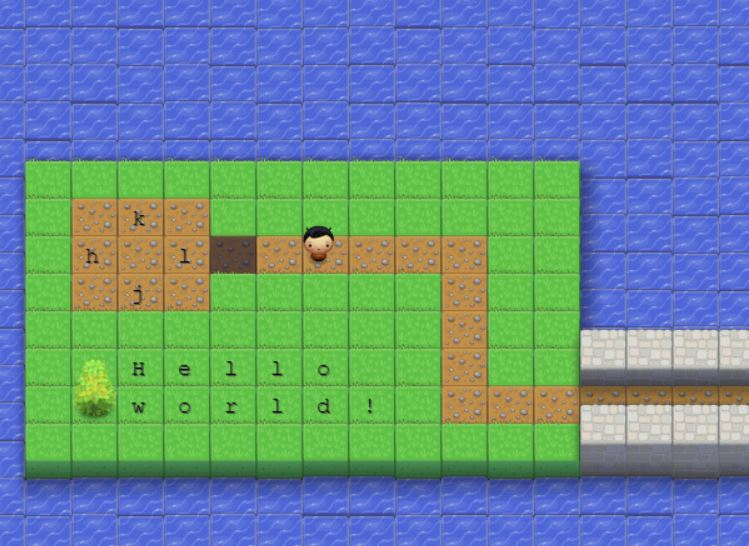
\includegraphics[width=0.6\textwidth]{vimadventures}
  \caption{\textit{Vim Adventures} Game Scene}
  \label{fig:vim-adventures}
\end{figure}

The value as a teaching tool lies inside the navigation commands for the player character. The controls for said navigation exactly match the navigation commands within the \textit{Vim} editor. While the player learns these commands (e.g., h,j,k,l keys for directional navigation as also shown in Figure \ref{fig:vim-adventures}) for in-game navigation these commands can simultaneously be used in the text editor. This allows for playful familiarization, possibly motivating the player/user to keep learning despite the steep learning curve of the editor itself. In conclusion, this example shows how a carefully crafted game can be able to provide educational value in a non-gaming context. Thus, this approach could act as a blueprint for a possible implementation of a technology-aided onboarding solution.

Another approach was taken by \textit{CodinGame} \footnote{\url{https://www.codingame.com/}, accessed on 14th of August, 2021}. \textit{CodinGame} is a mixture between an \gls{ide} and a game. It aims to educate developers on different programming languages and programming concepts. Within the \textit{CodinGame} environment, there are different tasks assigned to the player. These revolve around the visualization of the player character, game objects, and enemies on a part of the screen, as can be seen in \textit{Figure \ref{fig:codingame}}.

\begin{figure}[h]
  \centering
  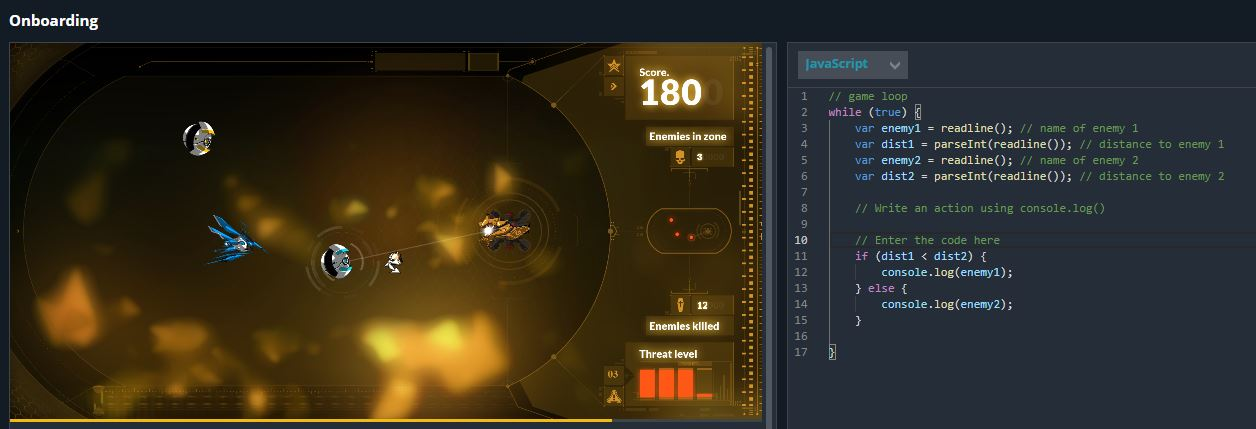
\includegraphics[width=0.9\textwidth]{codingame}
  \caption{\textit{CodinGame} Game Scene}
  \label{fig:codingame}
\end{figure}

Players then can tackle these tasks by writing valid source code in popular programming languages such as Javascript, C\#, C++, Java, and more. Within the source code, it is possible to reference the game objects entering the visualization on the other part of the screen. Through writing game-specific code you then are able to interact with these game objects (to kill the enemy objects for example). After the player has written the necessary code, it is possible to re-run the respective game scene and thus see if the task has been completed. Contrary to the previous example, \textit{CodinGame} does not try to teach concepts by matching mechanics to an outside concept. It rather uses writing source code as the central concept and only visualizes software development tasks playfully.

The \textit{Starbase} Game \footnote{\url{https://starbasegame.com/}, accessed on 14th of August 2021} represents another possible approach. Starbase is a massive multiplayer space adventure game. Unique to it, is its very detailed and intricate universe with a lot of different game mechanics and components to interact with. Instead of putting software development at the center or matching game mechanics to tool commands, \textit{Starbase} leverages software development in another way. Programming is used here as one of many game mechanics throughout the game. It allows for sophisticated control of in-game electrical devices. Code can be written in a custom programming language created specifically for the game. With that language, nearly every technological device within the game universe can be controlled. To summarize, programming or learning commands connected to programming is not a goal in itself in this case. Instead, it is used just as a single mechanic within a game, where it allows for extremely fine-grained control over in-game components.

In addition to these sample applications of play from the industry, there are also similar attempts in research. A recent example was created by Lopez et al., where the usage of LEGO\textregistered Serious play as an education tool for software development workflows was investigated. The study was set up in a way that students got handed a process definition to follow that matched popular project management techniques in software development. (e.g., a waterfall-style process and an agile process). Students then had to adhere to these processes with the overall goal to create a chair built out of LEGO\textregistered bricks. Depending on the given project management technique the process consisted of requirements, analysis, implementation, design, and evaluation phases in different orders. After students went through these phases, lecturers gave more context to these techniques and explained common pitfalls and advantages. Lopez et al. reported positive results within this study. Students were largely agreeing that it was highly fun and motivating to go through such processes playfully. The team environment together with lecturers acting as customers, allowed the students to hone their soft skills as well, as they reported. While this study does not resemble a game, it shows how toys can be appropriated into non-play contexts. This in turn allows for a playful learning experience, possibly increasing learning success \cite{lopez2021lego}.

Overall it can be said, that there is a great number of different approaches to utilizing the power of play in software development (or vice-versa, as shown with \textit{Starbase}) with different benefits gained from it. Within the implementation phase of the study, these different approaches could serve as possible implementation options. In essence, these options are:

\begin{itemize}
  \item{Leveraging commands or tools used in software development as key game mechanics -- similar to \textit{Vim Adventures}}
  \item{Using source code created by the player as the main way of interaction within a game -- similar to \textit{CodinGame}}
  \item{Using programming as one of many mechanics in a game -- similar to \textit{Starbase}}
  \item{Using toys or other elements of play to visualize or simulate non-gaming concepts -- similar to Lopez et al.'s approach}
\end{itemize}

Concerning using elements of play in the onboarding process of software development there is a lack of research. This reinforces the need for exploratory work into this exact topic, which ultimately is the goal of this thesis.

Lastly, after presenting these different approaches, there is one additional aspect of the software development context to clarify. The general openness towards integrating playful elements in such a process. A generalizable answer cannot be given, due to the large number of individual software developers already mentioned in this thesis' introduction. An attempt at answering the question can be made by investigating playful events and elements within the software development field. This could allow for an insight into the openness towards play.

One kind of those events are so-called \gls{ctf} contests. These have their origins in cybersecurity conventions. An example of such a contest would be the DefCon CTF\footnote{\url{https://defcon.org/html/links/dc-ctf.html}, accessed on 14th of August 2018}. Within such contests, teams of developers compete against each other by trying to compromise the other team's server. More specifically, teams are required \enquote{to leverage their knowledge of vulnerability detection} \cite[p. 134]{childers2010organizing} in order to attack and defend a virtualized host server. Points were then rewarded for both securing a team's own services but also compromising the enemy team's services \cite[p. 132-135]{childers2010organizing}. The competition as well as the special rule sets teams agree on, definitely resemble elements of play that were already mentioned.

Another kind of event, rising in popularity are so-called \textit{Hackathons}. These can be defined as:

\begin{quote}
  \textit{an event in which computer programmers and others involved in software development collaborate intensively over a short period of time on software projects [...]. These hackathons are encouraging of experimentation and creativity. and can be challenge orientated}

  \footnotesize{Gerard Briscoe, \cite[p. 1]{briscoe2014digital}}
\end{quote}

Briscoe describes that elements of hackathons originated from so-called \gls{lan} parties. These are gatherings \enquote{of people with computers or compatible computer game consoles} \cite[p. 3]{briscoe2014digital}. Therein one can see the playful origins of such events very clearly. But also the hackathons themselves show similar elements of play to the \gls{ctf} contests mentioned before with rule sets for the teams as well as possible competition. This holds true even more when looking at \textit{game jams}. These can be defined as \enquote{an accelerated opportunistic game creation event where a game is created in a relatively short timeframe} \cite{kultima2015defining}.

Besides those events, there also are signs of playfulness within the daily work of developers. While the coding work itself normally revolves around rather strict programming structures and syntaxes, playful elements can be discovered there as well. Uncovering all of those is out of scope for this thesis, so one exemplary element is going to be presented here. As a preface, it has to be understood how software developers collaborate on source code.

Typically, this is done with a version control system, where multiple developers are able to contribute code. This happens through aggregating changes in source code, then attaching a message and ultimately pushing the code changes to a place where other developers can access these changes and build upon them. The act of aggregating and attaching a message is called \textit{committing}. This is a central command within version control systems, as the attached messages communicate meta-information on the code changes to team members. This communication is usually held rather short and precise, but even within these commit messages, playful elements can be situated. An example for this is \textit{Gitmoji}\footnote{\url{https://gitmoji.dev}, accessed on 15th of August 2018}, a project that aims to include emojis within those commit messages. That usage of emojis, as Hjorth et al. point out:

\begin{quote}
  \textit{has been defined as playful (Sicart 2014 [original citation \cite{sicart2014play}]). This is epitomized by the playfulness of the paralinguistics -- emojis ('picture characters'), emoticons (typographic characters), stamps and stickers. [...] The use of paralinguistics has become an increasingly popular and playful way of personalizing digital media communications.}

  \footnotesize{Hjorth et al. \cite{hjorth2018beyond}}
\end{quote}

Overall one could assume that software developers might be open towards playful elements given the field's openness towards ludic features and events. These are not generalizable statements at this time, though. Therefore one of the additional goals of the upcoming study is to gather more data on exactly that attitude.

\subsection{Design Implications \& Attributes of Play}

After all the research done into possible theoretical foundations and related work in general, it is crucial to derive a set of attributes of play and possible design implications that inform the next chapters of this thesis. This is especially important for an informed study design. Consequently, this is going to be done in the following. Based on the literature that was analyzed beforehand, a non-exhaustive set of attributes is going to be derived. For each of these attributes, the theoretical grounding is presented as well. This is going to result in a list of attributes that inform playful design. These in turn serve as the foundation for further explorative research as is going to be laid out in chapter 3. The main theoretical grounding is derived from Miguel Sicart's \textit{Play Matters}, as it extends upon much of what came before in research into play. It also contains numerous actionable implications to explore further upon -- in contrast to equally as influential but more abstract and philosophical approaches like Suits' grasshopper. Where applicable, implications and attributes from other contemporary works are also included.

The first attribute of play is, that \textbf{play is a balance between creation and destruction}. This is based upon what Sicart describes as, \enquote{play is the struggle between order and chaos, between the will to create and destroy} \cite[p. 5]{sicart2014play}. This statement can very well be transformed into an actual playful feature of an onboarding experience into a software development project. As such, it is a prime candidate to explore further in the study that is following.

\textbf{Utilize already existing ludic features of a context} is the next implication from literature, based on Rodriguez \cite{rodriguez2006playful}. Some of these ludic features were described in chapter 2.3 and can be built upon during the study.

Rodriguez also proposes to \enquote{embrace conceptual uncertainty as a generative source [...] begin designing frameworks for actions that may or may not be considered playful} \cite{rodriguez2006playful}. When transferring that to an actual design implication, this can be interpreted as \textbf{embrace uncertain outcomes of playful elements}. That arguably is less of a directly actionable implication, rather a consideration to make. Nonetheless, it is a noteworthy addition to this list.

Another consideration Sicart mentions is that \enquote{play not as an activity of consumption but as as an activity of production […] play is a way of engaging and expressing our being in the world } \cite[p. 5]{sicart2014play}, which means that \textbf{play is an activity of production}.

Next up is an implication taken from a case study Sicart presented in \textit{play Matters}. There he describes the case of an application called \textit{The Accidental News Explorer}. It pulls random sources of news to show the user. Sicart describes it as a serendipitous approach, that \enquote{forces us to look at its choices with playful astonishment}. Thus, \textbf{utilize serendipitous events} can be included as a design implication.

Another crucial point brought up by Sicart is the idea of \enquote{disrupting the normal state of affairs by being playful [...] in that move, we reveal the inner workings of the context that we inhabit} \cite[p. 15]{sicart2014play}. This resonates extremely well with the overall goal of onboarding into software development projects. Within onboarding we want to reveal the inner workings of the project a developer is onboarded to, so there could be huge potential in applying Sicart's proposal to \textbf{disrupt the conventional state of affairs}.

One more implication with a lot of potentials based on the context at hand is described later on by Sicart, the idea that \enquote{creative appropriations of data reveal new knowledge through play [...] even in the most rigid of context} \cite[p. 28]{sicart2014play}. This points to playful visualizations of the context as a promising way to increase context-specific knowledge. Therefore the respective design implication would be, to \textbf{visualize creative appropriations of data}.

An additional implication -- also presented as a case study by Sicart -- is derived from \textit{Newstweek}. \textit{Newstweek} is an application that alters news headlines of major providers in real-time, \enquote{to playfully manipulate news consumption [...] shattering our assumptions on networks, news, and consumption of stories} \cite[p. 29]{sicart2014play}. \textbf{playfully manipulate the normal state of affairs} is, therefore, a design implication that can be derived here.

Sicart continues to propose elements of playful designs specifically. He mentions them being \enquote{by definition ambiguous, self-effacing, and in need for a user who will complete them} \cite[p. 31]{sicart2014play}. This can be directly translated into an implication of \textbf{Let the user complete intentionally ambiguous designs}. In the course of this argument, Sicart also mentions that what \enquote{playful design focuses on is the awareness of context as part of the design} \cite[p. 29]{sicart2014play}, so that is something to consider as well: \textbf{make the context a part of your playful design}. This also closely aligns to Bogost's statements on games as educational tools that are able to teach about certain concepts from a specific context.

\textbf{Create companions with personality}, is another design implication taken from Sicart's work. He specifically mentions this idea, while elaborating on Siri -- \enquote{Siri is a playful design that breaks our expectations and gives personality to software [...] Siri becomes a companion more than a tool} \cite[p. 32]{sicart2014play}.

Before tackling a larger subsection of implications, another noteworthy comment by Sicart is going to be considered. Within said comment, Sicart specifies that \enquote{playful designs could be described as somewhat successful toy designs, that is, as objects that by design allow users to toy around with them} \cite[p. 40]{sicart2014play}. Reconstructing that into a design implication makes for the statement of \textbf{think of designs as toys and let users freely play with them}.

Next up, the topic of \textit{procedurality} is mentioned numerous times by Sicart, who partly extends upon Bogost's work on procedural rhetoric. Therefore, multiple design implications can be inferred specifically on procedural designs. At first though, a short reminder on what those procedural systems are, they \enquote{generate behaviors based on rule-based models; they are machines capable of producing many outcomes, each conforming to the same overall guidelines} \cite[p. 4]{bogost2007persuasive}. In no particular order, these are the design implications derived for procedural systems as a whole and procedural toys specifically:

\begin{itemize}
  \item{\textbf{Allow the player to both watch the procedure unfold but also alter it} -- based on \enquote{procedural toys [...], are paradoxical objects that put their users in the double role of performer and voyeur [...] We play with them to see how they behave, how they react} \cite[p. 41]{sicart2014play}}
  \item{\textbf{Visualize the procedural world's conditions} -- based on \enquote{Procedural toys are mesmerizing because they are frames of the otherness, because they are tiny worlds that operate by their own condition} \cite[p. 43]{sicart2014play}}
  \item{\textbf{Let the player test the limits of the system} -- based on \enquote{Much of the joy in interacting with these procedural toys comes from testing their very propness as we figure out where the seams are and what we can build with them} \cite[p. 57]{sicart2014play}}
  \item{\textbf{Let the player explore and test without too much guidance} -- based on \enquote{Software toys like sim City and other procedural toys are also play spaces to a large extent -- spaces of possibility created to explore with rules in order to see what happens} \cite[p. 51]{sicart2014play}}
\end{itemize}

Moving on from procedural systems and toys, there are some more implications obtained from Sicart's statements. A statement that stood out was, that \enquote{designing for play means creating a setting rather than a system, a stage rather than a world, a model rather than a puzzle. Whatever is created has to be open, flexible, and malleable} \cite[p. 90]{sicart2014play}. This also resonates with the statement, that \enquote{the game designer proposes and deploys an object into the world, letting it speak for itself and be spoken through} \cite[p. 90]{sicart2014play}. Reconstructing that into an actual implication, would mean \textbf{treat the design as a deployable, flexible object rather than a polished piece}.

In addition to the design implications from literature on play, there were also some specific guidelines on onboarding experiences discovered through the extensive literature review. Similar to the play focused design implications these are laid out in a non-exhaustive list as follows:

\begin{itemize}
  \item{\textbf{Recommend specific (easy-to-achieve) tasks to beginners} -- based on \enquote{To promote early exploration, newcomers are often assigned small bug fixing tasks, chosen to introduce them to the code while minimising risks to the rest of the team; this is because maintenance is regarded as requiring less design knowlege than new feature development} (\cite{latoza2006maintaining} as cited in \cite[p. 36]{yates2014onboarding}) and \enquote{One way to make the path easier is to point newcomers to easy tasks} \cite[p. 8]{steinmacher2018let}}
  \item{\textbf{Recommend experienced mentors to newcomers} -- based on \enquote{experienced developers are key to understanding a project} \cite[p. 284]{dagenais2010moving} and \enquote{Identify mentors or experts} \cite[p. 9]{steinmacher2018let}}
  \item{\textbf{Visualize the micro and macro structure of projects} -- based on \enquote{ What about creating useful maps: micro and macro views that show the relationships between different landscape features and routes that can be taken} \cite[p. 284]{dagenais2010moving}}
  \item{\textbf{Document the code structure} as laid out by Steinmacher et al. \cite[p. 10]{steinmacher2018let}}
  \item{\textbf{Identify and dismiss outdated information} as laid out by Steinmacher et al. \cite[p. 10]{steinmacher2018let}}
\end{itemize}

That concludes the list of design implications derived from literature on both the context and research into play and playfulness. These implications can now be used as a foundation for the next step within this thesis. As such, they are going to serve as one of the anchor points for the explorative study design described in the following chapter.